\documentclass[a4paper,twocolumn]{article}

\usepackage[utf8]{inputenc}
\usepackage[T1]{fontenc}
\usepackage[acronym]{glossaries}
\usepackage{graphicx}
\usepackage{fullpage}
\usepackage{booktabs}
\usepackage{hyperref}
\usepackage{listings}
\usepackage{tablefootnote}
\usepackage{verbatim}
\usepackage{multirow}
\usepackage{subcaption}
\usepackage{floatrow}
\usepackage{siunitx}
\usepackage{wasysym}
\usepackage{natbib}
\usepackage{lipsum}
\usepackage{paralist}

\date{Fall semester 2017}

\newacronym{gps}{GPS}{Global Positioning System}
\newacronym{imu}{IMU}{Inertial Motion Unit}
\newacronym{uwb}{UWB}{Ultra Wide Band}


\title{Development of an ultra-wide band indoor positioning system}
\author{Antoine Albertelli}

\begin{document}
\maketitle
\pagenumbering{gobble}

\section{Context}

Absolute positioning is a required component in mobile robotics.
In outdoor applications, the \gls{gps} fulfills this goal.
However, its short wavelength prevents it from being used indoors.
Dead reckoning solutions such as \glspl{imu} or optic flow suffer from drift over time.
The goal of this project is to implement a low-cost indoor positioning solution based on \gls{uwb} modules.

\section{Working principle}

\begin{figure}[h!]
    \centering
    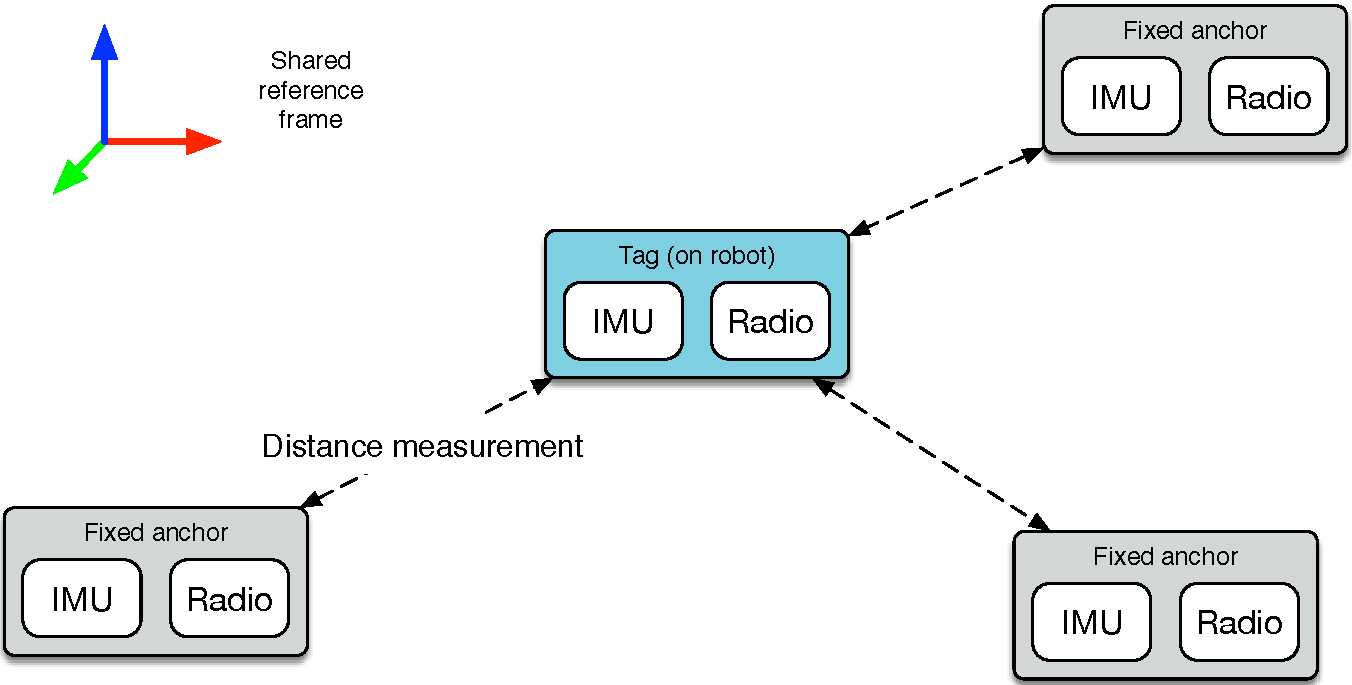
\includegraphics[width=\textwidth]{figures/system.pdf}
    \caption{Overview of the system, showing one mobile robot (blue) and three fixed anchors (grey).}
    \label{fig:system}
\end{figure}

The complete system (Figure~\ref{fig:system}) is made of two types of nodes, tags and anchors.
The distance between each node is obtained by measuring the time of flight for a radio packet.
The tags are placed on each robot, and estimate their position using the \gls{imu} combined with the distance measurements to the anchors.
The anchors are at a reference position (fixed) and can be used by several tags.
A tag will always use all the available anchors and will be able to seamlessly switch in case a tag is not in range anymore.

\section{Tasks}

After doing a review of the literature on the topic, I will start by doing a model of the system.
This includes both the dynamics of the system and the impact of noise on precision.
I should also investigate if the Digital Motion Processing unit built in the \gls{imu} can be useful.
I will then develop a position estimator taking the \gls{imu} data as inputs and the distance readings as measurements.

In parallel to this, I will write code for the reference board (Figure~\ref{fig:board}).
Several steps must be done in order to have a working system:
\begin{inparaenum}
    \item Drivers for the \gls{uwb} module and the \gls{imu} chip.
    \item Distance measurement protocol.
    \item Position estimation algorithm.
\end{inparaenum}

I will finish my work by measuring the performance of the system.
If time remains, I would like to implement a protocol to communicate over the \gls{uwb} link, to provide low bandwidth inter-robot communications without additional hardware.

\begin{figure}[h!]
    \centering
    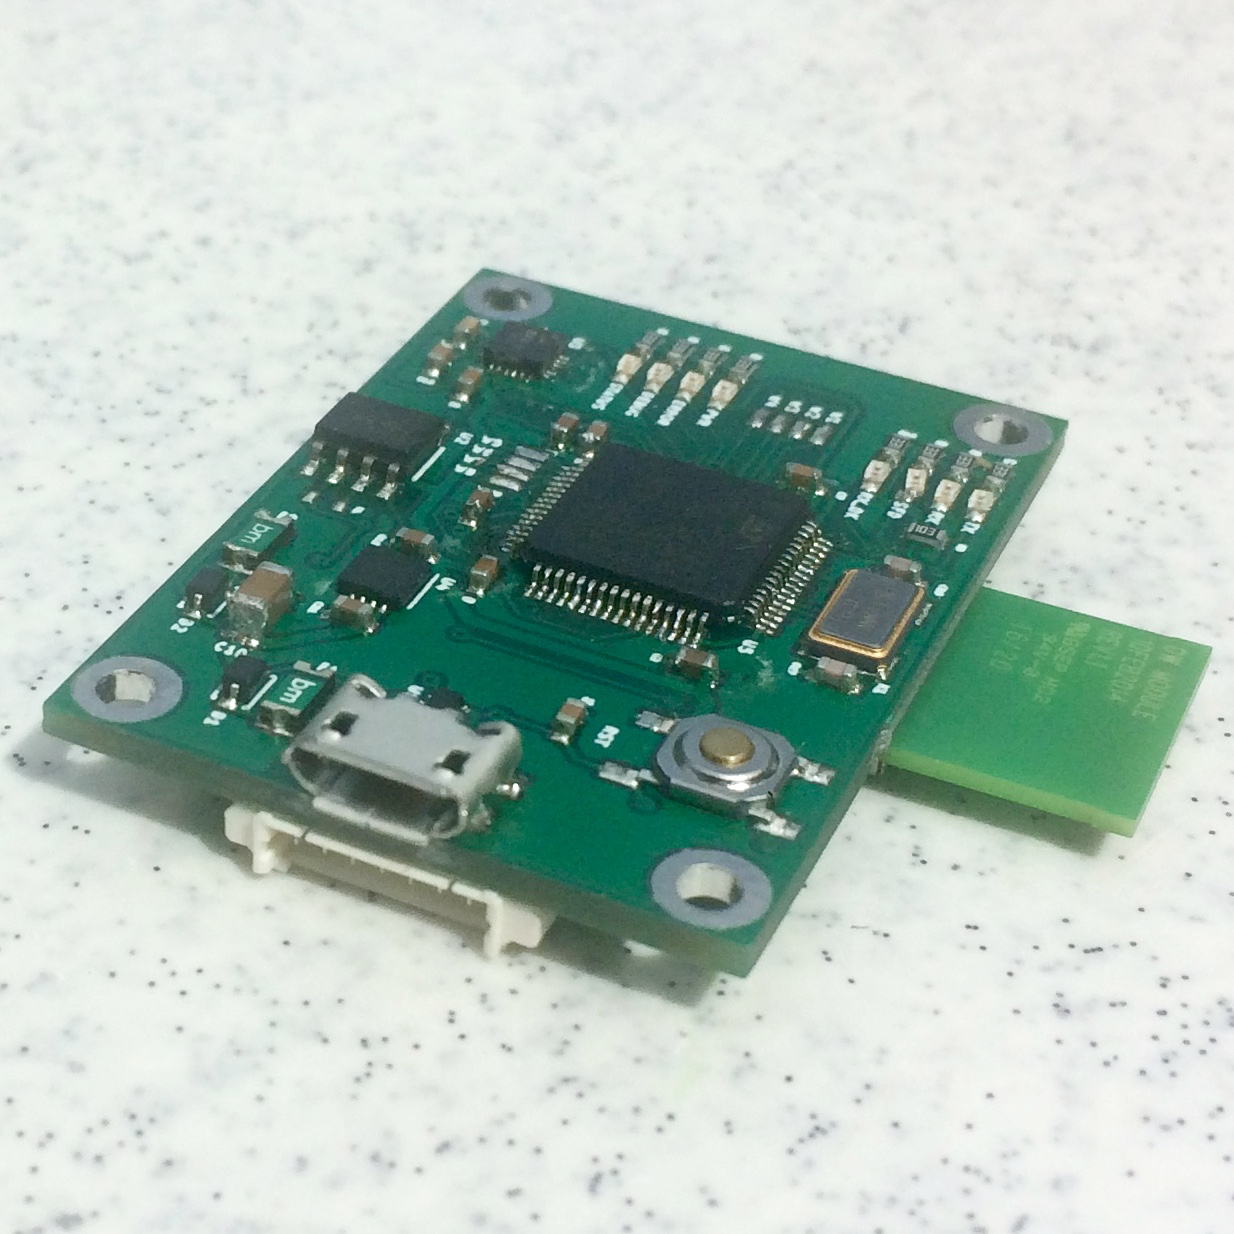
\includegraphics[width=0.4\textwidth]{figures/board}
    \caption{Reference board which includes an STM32F405 processor, a DWM1000 \gls{uwb} module and an MPU9250 \gls{imu}.}
    \label{fig:board}
\end{figure}

\section{Results}
\textbf{TODO}
\end{document}
